\section{Hibajavító Kódolás}

\begin{definicio}{Mézga Géza} Hamming távolság

	$d(\overline{a},\overline{b})$

	PL:
	\begin{displaymath}
    \
     \begin{array}{lr}
        \overline{a} = (01010) \\
       \overline{b} = (11111)
     \end{array} d(\overline{a},\overline{b}) = 3 = w(\overline{a} + \overline{b} )
   \
\end{displaymath}
\end{definicio}

\textbf{Alaptulajdonságok egyszerű Hamming kódnál:}
	\begin{enumerate}
		\item Lineáris kódnál $d_{min} = w_{min}$

		\item Ennyi 't' hiba javítható: $ t = \left\lfloor \dfrac{d_{min} -1}{2} \right\rfloor $

		\item Detektálható hiba: $d_{min} -1$

		\item MDS $\rightarrow$ $d_{min} = n-k+1$

	\end{enumerate}

\begin{tetel}{MZ/X használhatatlan cuccokat küld}
\textbf{Hamming egyenlőtlenség}

$$ \sum\limits_{i = 0}^t {n \choose i} \leq 2^{n-k} $$
\end{tetel}

Ha egyenlőség áll fent akkor \textbf{Perfekt kód}

\subsection{Szisztematikus kód}

\begin{definicio}{Mézga Géza}

Szisztematikus, ha minden kódszavra igaz hogy annak utolsó n-k szimbólumát elhagyva éppen a neki megfelelő k hosszúságú üzenetet kapjuk.
\end{definicio}

	\begin{enumerate}
		\item Generátor mátrix: $\MUnderline{G}_{k \times n} = \left( \MUnderline{E}_{k \times k} , \MUnderline{B} \right)$
		\item Paritásellenörző mátrix: $\MUnderline{H}_{(n-k)\times n} = \left( \MUnderline{A}_{(n-k)\times k} , \MUnderline{E}   \right)$
		\item $\MUnderline{A} = - \MUnderline{B}^T$

	\end{enumerate}

\subsection{Reid- Solomon (RS) kód}

	\begin{itemize}
		\item
\[
G_{k\times n}=
  \begin{pmatrix}
    1 & 1 & 1 & ... & 1 \\
    1 & \alpha & \alpha^2 & ... & \alpha^{n-1} \\
    1 & \alpha^2 & \alpha^4 & ... & \alpha^{2(n-1)} \\
    1 & ... & ... & ... & ...\\
    1 & \alpha^{k-1} & \alpha^{2(k-1)} & ... & \alpha^{(k-1)(n-1)}
  \end{pmatrix}
\]

%TODO H nembiztos hogy jó
\[
H_{(n-k)\times n}=
  \begin{pmatrix}
    1 & \alpha^1 & \alpha^2 & ... & \alpha^{n-1} \\
    1 & \alpha^2 & \alpha^4 & ... & \alpha^2{n-1} \\
    1 & ... & ... & ... & ...\\
    1 & \alpha^{n-k} & \alpha^{2(n-k)} & ... & \alpha^{(n-k)(n-1)}
  \end{pmatrix}
\]


	\item + Tetszőleges 't' hiba javítható
	\item + MDS
	\item + Real time bizonyos részek
	\item - LUT
	\item - q ális
	\item - GF(q) komplex

	\end{itemize}


\subsection{Shift regiszter típusok}

	\begin{enumerate}
		\item \textbf{Linear Feed Forward Shift Register (LFFSR) } - Előrecsatolt Shift Regiszter

		\item \textbf{Linear Feed Back Shift Register (LFBSR) } - Visszacsatolt Shift Regiszter
			\begin{center}
				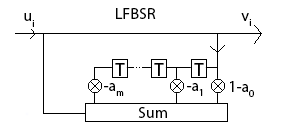
\includegraphics[scale=1]{img/LFBSR}
			\end{center}
		\item \textbf{Linear Feed Back Shift Register Wirth Remainder (LFFSR w.r) } - Visszacsatolt shift regiszter ( maradékos osztással)
			\begin{center}
				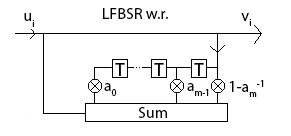
\includegraphics[scale=1]{img/LFBSRwr}
			\end{center}
	\end{enumerate}

\subsection{Ciklikus RS kód}

 	\begin{itemize}
 		\item $g(x) = \prod\limits_{i = 1}^{n-k} (x-\alpha^i)$
 		\item $h(x) = \prod\limits_{i = n-k+1}^{n} (x-\alpha^i)$
 	\end{itemize}

%TODO Hipacsapda alg
%TODO GF(2^n)
